\documentclass{beamer}

\mode<presentation>{
	%\usetheme{CambridgeUS}
	%\usecolortheme{seahorse}
	\usetheme{Boadilla}
	\usecolortheme{beaver}
	\setbeamertemplate{navigation symbols}{}
}

\usepackage{graphicx}
\usepackage{booktabs}
\usepackage{algpseudocode}
\usepackage{hyperref}
\usepackage{tikz}
\usepackage[utf8]{inputenc}
\usepackage{listings}
\usepackage[export]{adjustbox}
\usepackage{aeguill}

%\setbeamertemplate{title page}[default][rounded=false]

\setbeamertemplate{title page}
{
%\vbox{}
\begingroup
\centering
\begin{beamercolorbox}[sep=8pt,center]{institute}
\usebeamerfont{institute}\insertinstitute
\end{beamercolorbox}
\vskip1em%
\begin{beamercolorbox}[sep=8pt,center]{title}
\usebeamerfont{title}\inserttitle\par%
\ifx\insertsubtitle\@empty%
\else%
\vskip0.25em%
{\usebeamerfont{subtitle}\usebeamercolor[fg]{subtitle}\insertsubtitle\par}%
\fi%
\end{beamercolorbox}%
\vfill
\begin{beamercolorbox}[sep=8pt,center]{author}
\usebeamerfont{author}\insertauthor
\end{beamercolorbox}
\vskip1em\par
\begin{beamercolorbox}[sep=8pt,center]{date}
\usebeamerfont{date}\insertdate
\end{beamercolorbox}
\endgroup
}

\setbeamertemplate{blocks}[default]
\setbeamercolor{structure}{fg=darkred}
%\setbeamercolor{block title}{bg=darkred,fg=white}
%\setbeamercolor{block body}{bg=darkgray!20!white}
\setbeamercolor{block title}{bg=darkgray!30!white}
\setbeamertemplate{enumerate items}[default]

\setbeamertemplate{part page}{
\begin{beamercolorbox}[sep=8pt,center,wd=\textwidth]{part title}
\usebeamerfont{part title}\insertpart\par
\end{beamercolorbox}
\vfill
\tableofcontents
}

%\setbeamertemplate{frametitle continuation}{(\insertcontinuationcount)}

\setbeamertemplate{headline}{\leavevmode\hbox{\begin{beamercolorbox}[wd=.5\paperwidth,ht=2.65ex,dp=1.5ex,center]{section in head/foot}\usebeamerfont{section in head/foot}\insertsectionhead\hspace*{2ex}
\end{beamercolorbox}\begin{beamercolorbox}[wd=.5\paperwidth,ht=2.65ex,dp=1.5ex,center]{subsection in head/foot}\usebeamerfont{subsection in head/foot}\hspace*{2ex}\insertsubsectionhead\end{beamercolorbox}}\vskip0pt}

\setbeamertemplate{background}{\tikz[overlay,remember picture]\node[opacity=0.08]at (current page.south east){
\includegraphics[width=10cm]{figures/unibo_logo.jpg}};}

\newcommand{\tcc}[1]{\textcolor{darkred}{#1}}

\newcommand{\codeA}[1]{\texttt{#1}}
\newcommand{\codeB}[1]{\texttt{\textcolor{darkred}{#1}}}

\newcommand{\link}[1]{{\footnotesize » \url{#1}}}
\newcommand{\bothquote}[1]{``#1''}

\definecolor{mygreen}{rgb}{0,0.6,0}
\definecolor{mygray}{rgb}{0.5,0.5,0.5}
\definecolor{mymauve}{rgb}{0.58,0,0.82}
\definecolor{maroon}{rgb}{0.5,0,0}
\definecolor{darkgreen}{rgb}{0,0.5,0}

\lstset{
language=Java,
basicstyle=\scriptsize\ttfamily,
keywordstyle=\scriptsize\color{blue}\ttfamily,
commentstyle=\scriptsize\color{mygreen}\ttfamily,
breakatwhitespace=false,
breaklines=true,
 numbers=left,
  numberstyle=\color{mymauve},
  stringstyle=\color{mymauve},
  showstringspaces=false,
  numbers=none
}

\lstdefinelanguage{XML}
{
  basicstyle=\scriptsize\ttfamily,
  morestring=[s]{"}{"},
  morecomment=[s]{?}{?},
  morecomment=[s]{!--}{--},
  commentstyle=\color{darkgreen},
  moredelim=[s][\color{black}]{>}{<},
  moredelim=[s][\color{red}]{\ }{=},
  stringstyle=\color{blue},
  identifierstyle=\color{maroon},
  numbers=none
}

\makeatother

\AtBeginSection[]
{
  \begin{frame}
    \frametitle{Outline}
    \tableofcontents[currentsection]
  \end{frame}
}

%\AtBeginSubsection[]
%{
%  \begin{frame}
%    \frametitle{Outline}
%    \tableofcontents[currentsection,currentsubsection]
%  \end{frame}
%}

\institute[UNIBO]{\uppercase{Alma Mater Studiorum -- Università di Bologna}\\Dipartimento di Informatica -- Scienza e Ingegneria (DISI)\\C.d.S. in Ingegneria e Scienze Informatiche, Campus di Cesena}

\author[A. Marfoglia]{Alberto Marfoglia\\\scriptsize\texttt{alberto.marfoglia2@unibo.it}}


\title[Android -- 1B -- Activity]{Android Programming}
\subtitle{Activity}
\date[ver. 1.0 (20220505)]{Embedded Systems and Internet of Things\\A.A. 2021 -- 2022}

\begin{document}

\begin{frame}
\titlepage
\end{frame}

\newcommand\blfootnote[1]{%
  \begingroup
  \renewcommand\thefootnote{}\footnote{#1}%
  \addtocounter{footnote}{-1}%
  \endgroup
}

\begin{frame}{Thanks}
    \centering
    \begin{itemize}
      \item \large{Professor Angelo Croatti}
    \end{itemize}

    \blfootnote{\url{https://www.unibo.it/sitoweb/a.croatti/en}}
    \blfootnote{}
\end{frame}

\section{Overview}

\begin{frame}{Activity}
  \begin{block}{Overview}
    \begin{itemize}
      \item An activity is the entry point for interacting with the user.
      \item Unlike other paradigms, in the case there is no \codeA{main} function.
      \item An application can be seen as a collection of interconnected activities.
      \item Typically, one activity in an app is specified as the \tcc{main} activity.
    \end{itemize}
  \end{block}
  \begin{exampleblock}{Example}
    \lstinputlisting[language=XML]{./code/main-activity-example.xml}
  \end{exampleblock}
\end{frame}

\begin{frame}{Activity: Android App Example}
\begin{figure}
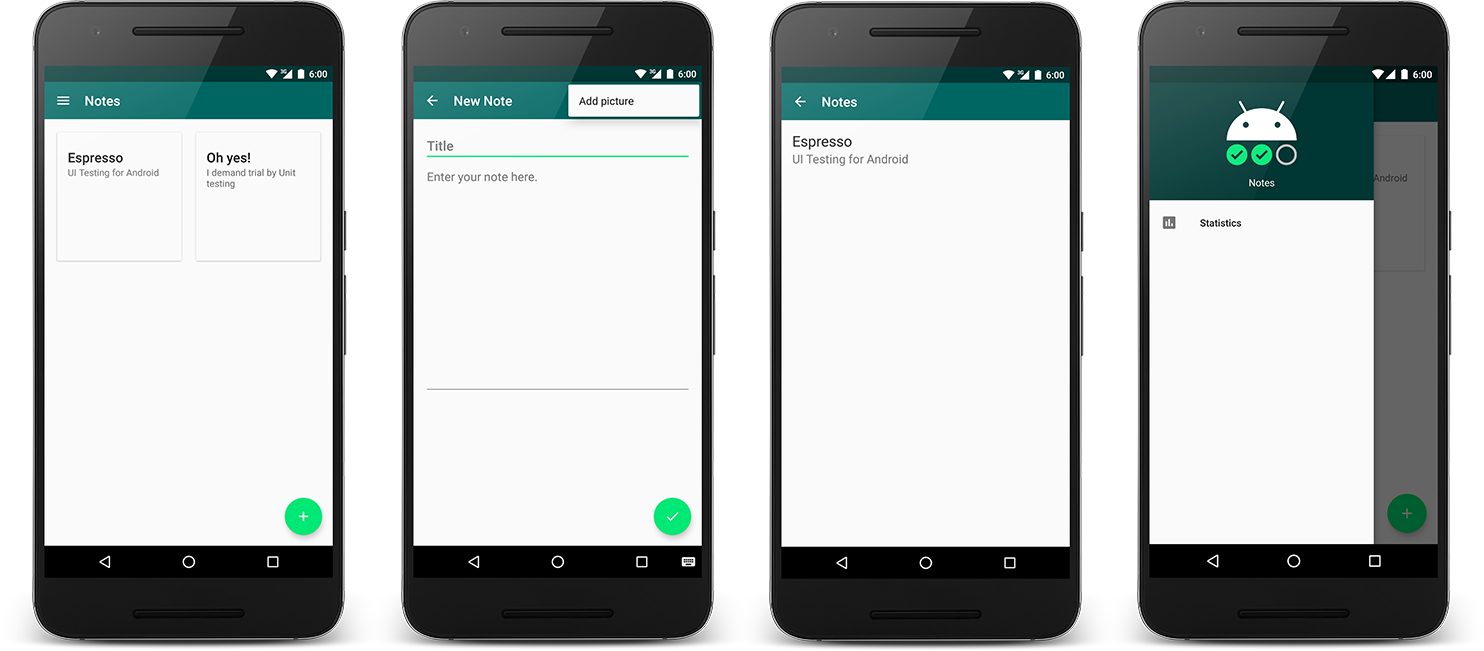
\includegraphics[width=\linewidth]{figures/activity-ex.png}
\end{figure}
\end{frame}

\section{Activity Lifecycle}

\begin{frame}[fragile, allowframebreaks]{Activity Lifecycle}
  \begin{block}{Lifecycle}
    \begin{itemize}
      \item The lifecycle is made up of a set of states and internal loops.
      \item The Activity class provides a number of callbacks that allow the activity to know that a state has changed.
      \begin{itemize}
        \item Especially: \codeB{onCreate()}, \codeB{onStart()}, \codeB{onPause()}, \codeB{onDestroy()}.
      \end{itemize}
    \end{itemize}
  \end{block}

  \begin{block}{Activity Status}
    \begin{itemize}
      \item \tcc{RUNNING}: the activity is in foreground and has the focus.
      \item \tcc{PAUSED}: the activity is still visible but it doesn't have the focus.
      \item \tcc{STOPPED}: the activity is in background as it obscured by another.
    \end{itemize}
  \end{block}

  {\small \textbf{NOTE}: The system can remove a STOPPED or PAUSED activity at any time.}

  \begin{block}{Lifecycle Management}
    A good implementation of the lifecycle callbacks avoid:
    \begin{itemize}
      \item Crashing if the user switches to another app.
      \item Consuming valuable system resources when the user is not actively using it.
      \item Losing the user's progress if they leave the app and return it at a later time.
      \item Crashing or loosing the user's progress when the screen rotates.
    \end{itemize}
  \end{block}

  \begin{figure}
    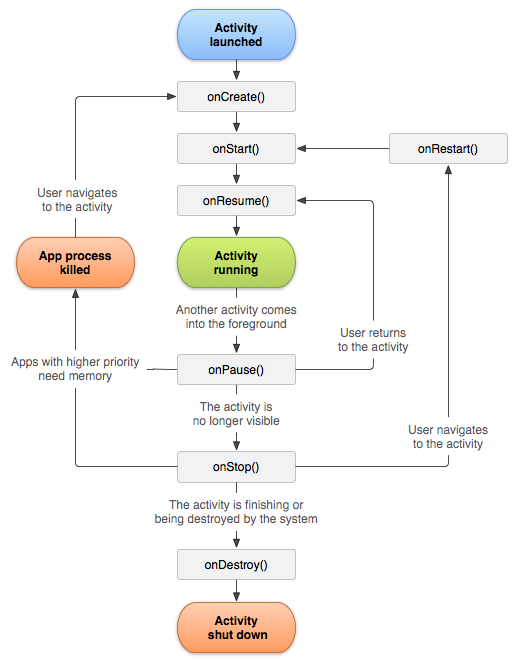
\includegraphics[width=0.5\textwidth]{figures/activity_lifecycle.png}
  \end{figure}
\end{frame}

\subsection{Callbacks}

\begin{frame}[allowframebreaks]{Activity Lifecycle -- Callback}
% \begin{itemize}
% \item \textbf{La ridefinizione di ciascuna callback deve obbligatoriamente richiamare l'implementazione originale corrispondente.}
% \begin{itemize}
% \item Es.: La ridefinizione del metodo \codeA{onStart()} in una propria activity deve richiamare nel suo corpo lo stesso metodo definito nella super-class \codeA{Activity} con l'istruzione \codeA{super.onStart()}.
% \end{itemize}
% \end{itemize}
  \begin{block}{Before start}
    Overriding each callback must invoke the corresponding original implementation.
    \begin{itemize}
      \item Ex. the \codeA{onStart()} redefinition involves calling the \codeB{super}\codeA{.onStart()}
    \end{itemize}
  \end{block}

  \begin{block}{\codeB{onCreate(Bundle savedInstanceState)}}
    \begin{itemize}
      \item It fires when the system first create the activity.
      \item It provides for the setup of activity, it's performed only once.
      \item It receives any previously saved state from the system.
    \end{itemize}
  \end{block}

  \newpage

  \begin{block}{\codeB{onStart()}}
    \begin{itemize}
      \item It is invoked just before the activity is made visible to the user.
      \item Prepares the activity so that it can be place in foreground.
    \end{itemize}
  \end{block}

  \begin{block}{\codeB{onResume()}}
    \begin{itemize}
      \item It triggers when the activity comes to foreground.
      \item At end of its execution, the activity is in the RUNNING state.
    \end{itemize}
  \end{block}

  \begin{block}{\codeB{onStop()}}
    \begin{itemize}
      \item It fires when the activity is no longer visible to the user.
      \item At end of its execution, the activity is in the STOPPED state.
    \end{itemize}
  \end{block}

  \begin{block}{\codeB{onPause()}}
    \begin{itemize}
      \item It is called from the system when the user is leaving the activity.
      \item Generally used to release any resources held by the activity, but not only:
      \begin{itemize}
        \item A new activity open (such as a dialog)
        \item In Android 7.0 or higher, multiple apps run in multi-window mode
        \item Some event interrupts app execution
      \end{itemize}
      \item At the end of its execution, the activity is in the PAUSED state.
    \end{itemize}
  \end{block}

  \begin{block}{\codeB{onRestart()}}
    \begin{itemize}
      \item It is invoked by the system when a previously stopped activity comes back.
    \end{itemize}
  \end{block}

  \begin{block}{\codeB{onDestroy()}}
    \begin{itemize}
      \item It is called just before the activity is destroyed.
      \item It can be fired either by the user or by the system.
      \begin{itemize}
        \item \textbf{Generally, the termination of the activities is delegated to the system}.
      \end{itemize}
    \end{itemize}
  \end{block}

\end{frame}

\section{Activity Management}
  \subsection{Creation}

  \begin{frame}[fragile,allowframebreaks]{Activity Creation}
    \begin{block}{Mandatory steps}
      \begin{itemize}
        \item Each activity must be defined as a subclass of \tcc{android.app.Activity}
        \item It must necessarily implement the \codeB{onCreate()} method.
        \begin{itemize}
          \item You must invoke method \tcc{setContentView(int resID)} to associate the resource that defines the UI with the activity.
        \end{itemize}
      \end{itemize}
    \end{block}

    \begin{block}{Other notes}
      \begin{itemize}
        \item The implementation of method \codeB{onPause()} is considered a best practice.
        \begin{itemize}
          \item This is where resources are usually released.
        \end{itemize}
        \item The implementation of all other callbacks is optional.
      \end{itemize}
    \end{block}
    
    \begin{exampleblock}{Example}
      \lstinputlisting[language=Java]{./code/activity-example.java}
    \end{exampleblock}

    \begin{itemize}
      \item Remember, each activity has to be declared inside the Manifest File.
    \end{itemize}
  \end{frame}
  % \newpage

  % \begin{itemize}\itemsep5pt
  %   \item Ciascuna activity \underline{deve} essere dichiarata nel File Manifest.
  %   \begin{itemize}
  %     \item Deve necessariamente essere specificato un valore per l'attributo \codeB{android:name}, che deve contenere il nome completo della classe.
  %     \item Possono essere aggiunti altri parametri per la configurazione dell'activity.
  %   \end{itemize} 
  % \end{itemize} 
  % \begin{exampleblock}{Esempio}
  % \begin{lstlisting}[language=XML]
  % <manifest> <!-- Manifest tag properties omitted -->
  %   <application>
  %     <activity
  %       android:name="com.example.MyActivity"
  %       android:label="@string/app_name"/>
  %   </application>
  % </manifest>
  % \end{lstlisting}
  % \end{exampleblock}
  % \end{frame}

  \begin{frame}[fragile]{Main Activity declaration}
    \begin{itemize}
      \item Among the activities specified in the File Manifest, one of these must be labeled as 
      \tcc{Main Activity}, specifying a default Intent Filter
    \end{itemize}

    \begin{exampleblock}{Example}
      \lstinputlisting[language=xml]{./code/main-activity-example.xml}
    \end{exampleblock}
  \end{frame}

\subsection{Startup}

  \begin{frame}[fragile]{Activity: Start up}
    The activity class provides the \codeB{startActivity(Intent intent)} method used to start another activity.
    \begin{itemize}
      \item The intent is created by explicitly passing the reference to the \textit{activity} to be started.
      \item It may contain config. params (\tcc{flags}) or data to transmit (\tcc{extras}).
    \end{itemize}
    \begin{exampleblock}{Example -- Start \codeA{NewActivity}}
      \lstinputlisting[language=java]{./code/intent-creator-example.java}
    \end{exampleblock}

    \begin{exampleblock}{Example -- Recovery of trasmetted data}
      \lstinputlisting[language=java]{./code/intent-recovery-example.java}
    \end{exampleblock}
  \end{frame}

  \begin{frame}[fragile,allowframebreaks]{Activity: Start up (with result)}
    \begin{block}{How to start an activity for result}
    \begin{itemize}\itemsep10pt
      \item It may be necessary to start an activity whose result is \underline{propagated back to the calling activity}.
      \item You must use the \codeB{startActivityForResult(Intent intent, int reqID)} method, associating an arbitrary ID to the request.
    \end{itemize}
  \end{block}

  \begin{block}{How to retrive the result}
    \begin{itemize}\itemsep10pt
      \item In order to intercept th result must be implemented the \codeB{onActivityResult()} method.
      \begin{itemize}
        \item It's called by the system whenever the result is available.
      \end{itemize}
    \end{itemize}
  \end{block}

  \newpage
  \begin{exampleblock}{Example -- \codeA{CheckLoginActivity}}
    \lstinputlisting[language=java]{./code/check-login-activity.java}
  \end{exampleblock}

  \begin{itemize}
    \item The result produce by the activity can be back propagated via an \textit{intent}.
    \begin{itemize}
      \item You add the necessary \textit{extras}
      \item You must invoke \codeB{setResult(int resCode, Intent data)} before the activity termination.
      \item Possible types of results: \codeB{RESULT\_OK}, \codeB{RESULT\_CANCELED}, \dots
    \end{itemize}
  \end{itemize}


  \begin{exampleblock}{Example -- Return of the result}
    \lstinputlisting[language=java]{./code/activity-return-of-result.java}
  \end{exampleblock}

\end{frame}

\section{Back Stack}

\begin{frame}[allowframebreaks]{Activity Back Stack}
  \begin{itemize}
    \item Usually an application is composed of several activities.
    \begin{itemize}
      \item Only one can be visibile to the user (RUNNING state).
      \item The others are arranged in a stack LIFO called \tcc{Back Stack}.
    \end{itemize}
    \item If the user presses Back, the current activity is popped off the stack.
    \item At the base of the stack there's always the Home Screen.
  \end{itemize}

  \begin{figure}
    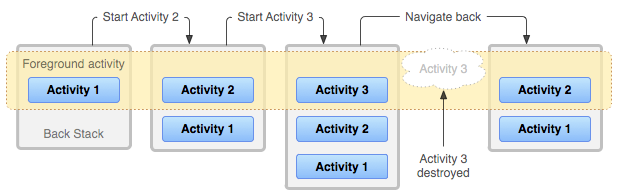
\includegraphics[width=1\linewidth]{figures/diagram_backstack.png}
  \end{figure}

\end{frame}

\section*{Riferimenti}
%-----------------------
%--- ONLINE RESURCES ---
%-----------------------

\begin{frame}{References - Online Resources}
\begin{thebibliography}{99}
\setbeamertemplate{bibliography item}[online]

\bibitem{adAPIguide} Android Developers - Guide
\newblock \link{https://developer.android.com/guide/}

\bibitem{adAPIreference} Android Developers - API Reference
\newblock \link{https://developer.android.com/reference/}

\bibitem{adTraining} Android Developers - Samples
\newblock \link{https://developer.android.com/samples/}

\bibitem{adTraining} Android Developers - Design \& Quality
\newblock \link{https://developer.android.com/design/}

\end{thebibliography}
\end{frame}

%-----------------------
%--- BOOKS -------------
%-----------------------

%\begin{frame}{Riferimenti - Libri}
%\begin{thebibliography}{99}
%\setbeamertemplate{bibliography item}[book]
%
%\bibitem{Mednieks11} Zigurd Mednieks, Laird Dornin, G. Blake Meike, Masumi Nakamura
%\newblock \emph{Programming Android}
%\newblock O'Reilly, 2011
%
%\bibitem{Haseman13} Chris Haseman, Kevin Grant
%\newblock \emph{Beginning Android Programming: Develop and Design}
%\newblock Peachpit Press, 2013
%
%\bibitem{Schwarz13} Ronan Schwarz, Phil Dutson, James Steele, Nelson To
%\newblock \emph{The Android Developer's Cookbook : Building Applications with the Android SDK}
%\newblock Addison-Wesley, 2013 
%
%\bibitem{Neil14} Theresa Neil
%\newblock \emph{Mobile Design Pattern Gallery: UI Patterns for Smartphone App}
%\newblock O'Relly, Second Edition, 2014
%\end{thebibliography}
%\end{frame}

\end{document}
